\documentclass{article}

% Chinese Support using xeCJK
% \usepackage{xeCJK}
% \setCJKmainfont{SimSun}

% Chinese Support using CTeX
% \usepackage{ctex}

% Math Support
\usepackage{amsmath}
\usepackage{amsfonts}
\usepackage{amssymb}
\usepackage{wasysym}

% Graphics Support
\usepackage{graphicx}
\usepackage{float}

% Reduced page margin
\usepackage{geometry}
\geometry{a4paper,scale=0.8}

\usepackage{caption}
\usepackage{subcaption}

% d and e should be math operators
\newcommand*{\dif}{\mathop{}\!\mathrm{d}}
\newcommand*{\md}{\mathop{}\!\mathrm{d}}
\newcommand*{\me}{\mathrm{e}}

% No indent for each paragraph
\usepackage{parskip}
\setlength{\parindent}{0cm}

% Bold style for Greek letters
\usepackage{bm}
\let\Oldmathbf\mathbf
\renewcommand{\mathbf}[1]{\boldsymbol{\Oldmathbf{#1}}}

% More space for dfrac in cell
\usepackage{cellspace}
\setlength{\cellspacetoplimit}{5pt}
\setlength{\cellspacebottomlimit}{5pt}

% SI units
\newcommand{\si}[1]{\  \mathrm{#1}}

% Multi-line author information
\usepackage{authblk}
\author{Xiping Hu}
\affil{https://hxp.plus/}

\title{Homework for Chapter 10}

\begin{document}

\maketitle

\begin{figure}[H]
  \centering
  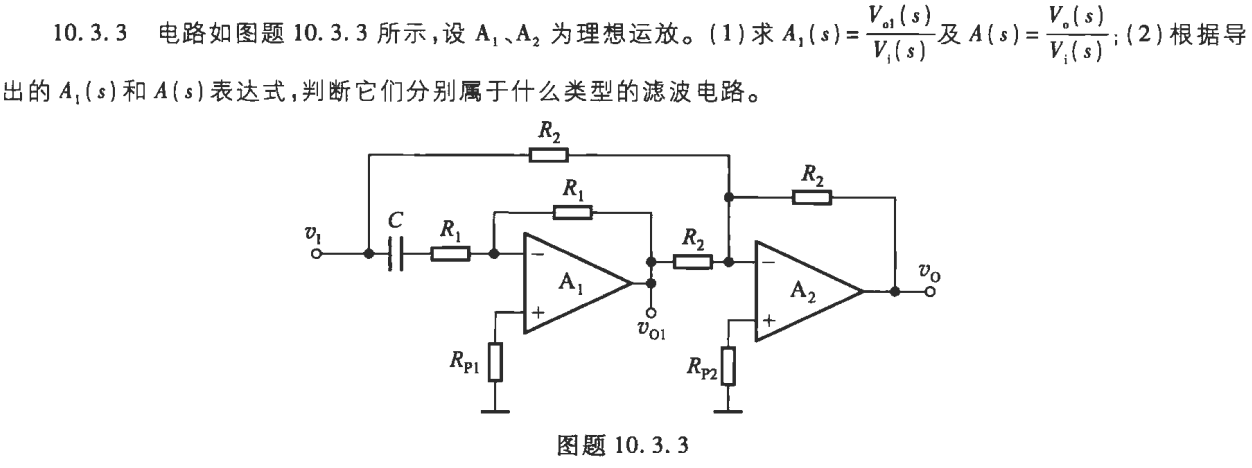
\includegraphics[width=\linewidth]{figures/Problem1033}
\end{figure}

\section{Problem 1}

\begin{equation*}
  \begin{aligned}
    A_1 \left( s \right) &= - \dfrac{R_1}{R_1 + \dfrac{1}{j \omega C} } = \dfrac{v_{o1} \left( s \right)}{v_1 \left( s \right)}  \\
    v_0 \left( s \right) &= - \dfrac{R_2}{R_2} v_{o1} - \dfrac{R_2}{R_2} v_1 = - v_{o1} - v_1 \\
    A \left( s \right) &= \dfrac{v_o}{v_1} = - \dfrac{v_{o1} + v_1}{v_1} = \dfrac{R_1}{R_1 + \dfrac{1}{j \omega C} } - 1 = - \dfrac{\dfrac{1}{j \omega C} }{R_1 + \dfrac{1}{j \omega C} }  = - \dfrac{1}{1 + j \omega C R_1} 
  \end{aligned}
\end{equation*}

\section{Problem 2}

$A_1$ is low-pass filter while $A$ is low-pass filter as well.

\end{document}